\section{Dynamic Structural Graph Operations}
\label{sec:eval:dynamic}

% TODO: Update spider chart — merge Insert Tput / Update Tput into a single
% "Ingest/Update" axis and add a "Dynamic OLAP" axis (geomean or sum of
% BFS+PR+WCC on graph500-26).

Dynamic graph processing systems target high-performance
ingest and operate primarily in memory.
We use three such systems to establish a baseline:
Teseo~\cite{teseo2021deLeo}, LiveGraph~\cite{zhu2019livegraph}, and
GraphOne~\cite{graphone2019kumar}.
Each system achieves high ingest throughput through lightweight write paths.
GraphOne appends edges to a lock-free ring buffer that a background archiver drains asynchronously.
Teseo inserts edges in-place into sorted segments of a fat tree under optimistic latches, attaching version records only to modified entries.
LiveGraph appends timestamped edge entries into per-vertex mmap-backed blocks.
% None of the three exports the graph to a separate analytics engine; each serves kernels from its own structures, though their read paths differ.
GraphOne's archiver drains the log into per-vertex adjacency chains in a read-optimized store; analytics waits for the archiver to finish, then reads each vertex's chain into a flat array with no per-edge version checks.
Teseo scans its sorted segments sequentially under optimistic latches; clean segments skip version checks entirely, while dirty ones consult a sparse undo log.
LiveGraph iterates each vertex's edge block under snapshot isolation, filtering every entry against the read epoch with two timestamp comparisons.


Most dynamic graph systems (such as ASPEN~\cite{10.1145/3314221.3314598}, STINGER~\cite{stinger2012ediger}, Sortledton~\cite{sortledton2022Fuchs}, and GTX~\cite{libinzhou2025GTX}) have no way to persist data across restarts; the exceptions are LiveGraph~\cite{zhu2019livegraph}, which supports file-backed mmap, and GraphOne~\cite{graphone2019kumar}, which provides a write-ahead log.
For a fair comparison with Teseo~\cite{teseo2021deLeo}, we disable persistence in LiveGraph and GraphOne, so all three baselines operate under comparable in-memory conditions.
Recall that \project{} is inherently persistent; to best approximate in-memory behavior in the presence of updates, we disable the write-ahead log and checkpointing and size \wt{}'s cache to prevent most evictions.
We do not use \wt{}'s in-memory mode, because it would be contrary to our design objective.
We therefore avoid as much disk I/O as possible, but \project{} still maintains the graph in \wt{}'s persistable, page-oriented B-tree format at all times.
We call the CPU cost of maintaining that format the \textbf{\emph{persistence machinery tax}}: not the cost of persisting data, but of keeping a structure that is persistable by construction.
The machinery consists of byte-comparable key serialization, disk-block-granular page geometry, page-image reconciliation, extent/block management, and an always-on eviction subsystem.
It excludes write-ahead logging and checkpointing, which are turned off unless noted otherwise.
\autoref{sec:wt-ingest-overhead} measures what the tax costs on the ingest path.
GraphOne and LiveGraph decouple durability from their in-memory representation and pay essentially nothing for the option.
These designs have consequences, however: GraphOne enforces no transactional consistency during updates.
It delegates duplicate checking to the caller; its snapshot mechanism is too heavyweight to invoke per-edge, and throughput collapses if used that way.
Teseo provides transactional semantics comparable to \project{}'s, but it has no durable representation and incurs no persistence overhead.
LiveGraph has similar transactional semantics, but since it relies on mmap, the host OS can evict pages at any time, so the write ordering needed for consistency and crash recovery is difficult, if not impossible, to guarantee.

We conduct four experiments:
(1)~a scalability study that varies writer thread count,
(2)~an insertion benchmark at each system's optimal thread count,
(3)~a sustained mixed insert-and-delete workload that replays a graph
update log,
(4)~a graph analytics benchmark (PageRank, BFS, and weakly connected components) run on the graph each system holds once the insertion-only ingest of~(2) completes.

%%%%%%%%%%%%%%%%%%%%%%%%%%%%%%%%%%%%%%%%%%%%%%%%%%%%%%%%%%%%%%%%%%%%%%%%%%%%%%%%
% TODO: regenerate as a single-column, single-panel figure (scalability only;
% drop the peak-throughput bar chart — those numbers are now in the prose).
\begin{figure*}[ht]
  \centering
  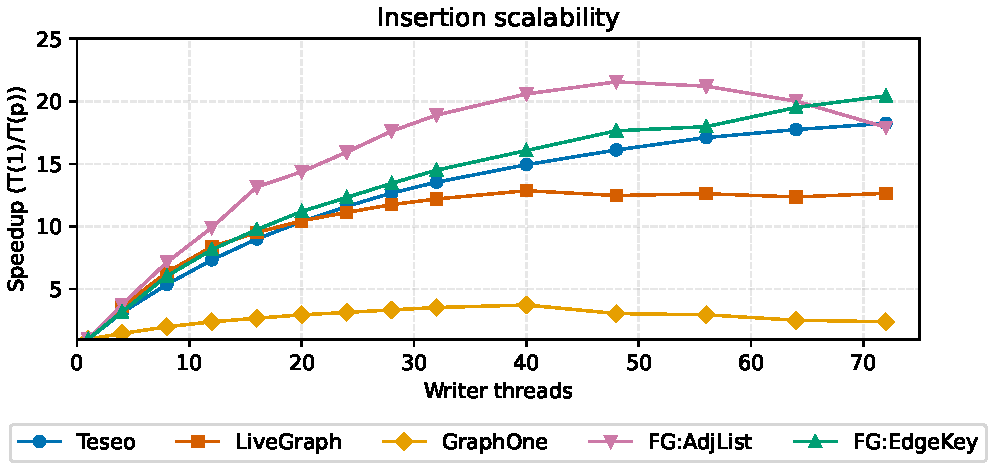
\includegraphics[width=\textwidth]{fig/dynamic/scalability.pdf}
  \caption{Insertion scalability with increasing writer thread count on graph500-24.
  Each line is relative to its own single-thread baseline, so the figure does not show
  relative performance between the systems; \autoref{tab:scalability-peak} gives the
  absolute throughputs.}
  % (b)~peak insertion throughput across datasets,
  \label{fig:dynamic-scaling}
\end{figure*}
%%%%%%%%%%%%%%%%%%%%%%%%%%%%%%%%%%%%%%%%%%%%%%%%%%%%%%%%%%%%%%%%%%%%%%%%%%%%%%%%

\section{Insertion Scalability}
\label{sec:eval:dynamic:scalability}
\newflag[new peak-throughput table]

We insert the edges of graph500-24 while varying the number of writer threads from 1 to 72 to identify each system's optimal concurrency (\autoref{fig:dynamic-scaling}).
\autoref{tab:scalability-peak} lists each system's single-thread and peak throughput.
GraphOne peaks at 6.33\,M~edges/s with 40~threads but degrades beyond that point as cross-socket contention on its single ring buffer increases.
Teseo scales the most consistently, reaching 5.12\,M~edges/s at 72~threads with no sign of saturation.
LiveGraph plateaus near 0.49\,M~edges/s at 32--40~threads.
\project{} EdgeKey reaches 1.69\,M~edges/s at 72~threads; Adjacency List peaks at 0.83\,M~edges/s with 48~threads.

\project{} is not competitive with the in-memory systems on raw insertion throughput, and the table illustrates the gap: \project{} EdgeKey's peak of 1.69\,M~edges/s at 72~threads is exactly GraphOne's single-thread throughput.
At one writer \project{} trails GraphOne by 24$\times$; at peak it trails GraphOne by 3.7$\times$ and Teseo by 3.0$\times$.
The deficit is structural; \autoref{sec:dynamic:ingest-update-tput} discusses where the time goes.
Neither \project{} configuration has saturated at 72~threads, so the gap narrows as concurrency rises, but it does not close.

Based on these results, we fix GraphOne and LiveGraph at 40~threads, \project{}'s AdjList configration at 48~threads, and Teseo and \project{}'s EdgeKey configurations at 72~threads for all subsequent experiments.

%%%%%%%%%%%%%%%%%%%%%%%%%%%%%%%%%%%%%%%%%%%%%%%%%%%%%%%%%%%%%%%%%%%%%%%%%%%%%%%%
\begin{table}[t]
  \centering
  \small
  \setlength{\tabcolsep}{5pt}\renewcommand{\arraystretch}{1.05}
  \begin{tabular}{l r r c r}
  \toprule
  System
    & \begin{tabular}[b]{@{}r@{}}Meps at\\1 thread\end{tabular}
    & \begin{tabular}[b]{@{}r@{}}Meps at\\$p$ threads\end{tabular}
    & \begin{tabular}[b]{@{}c@{}}$p$\\(peak threads)\end{tabular}
    & Speedup \\
  \midrule
  GraphOne              & \textbf{1.69} & \textbf{6.33} & 40 & 3.7$\times$ \\
  Teseo                 & 0.28 & 5.12 & 72 & 18.2$\times$ \\
  \project{} EdgeKey    & 0.07 & 1.69 & 72 & \textbf{23.5}$\times$ \\
  \project{} AdjList    & 0.04 & 0.83 & 48 & 21.3$\times$ \\
  LiveGraph             & 0.04 & 0.49 & 40 & 12.9$\times$ \\
  \bottomrule
  \end{tabular}
  \caption{Single-thread and peak insertion throughput on graph500-24, in millions of
  edges per second (Meps).
  $p$ is the thread count at which each system peaks, and speedup is its peak throughput
  divided by its single-thread throughput.
  The best value in each column appears in bold.}
  \label{tab:scalability-peak}
\end{table}
%%%%%%%%%%%%%%%%%%%%%%%%%%%%%%%%%%%%%%%%%%%%%%%%%%%%%%%%%%%%%%%%%%%%%%%%%%%%%%%%

\section{Ingest and Update Throughput}
\label{sec:dynamic:ingest-update-tput}

Having identified optimal thread counts, we next examine ingest and sustained update performance.
\autoref{fig:throughput-all} shows insertion-only throughput across six datasets (51\,M to 1.05\,B edges).
GraphOne and Teseo are substantially faster than \project{}, sustaining 5.6--6.6 and 4.3--5.5\,M~edges/s respectively, 3 to 5$\times$ faster than \project{} EdgeKey (1.2--1.8\,M~edges/s).
\project{} EdgeKey is $3\times$ faster than LiveGraph (0.48\,M~edges/s).
GraphOne issues blind writes and performs no existence checks during inserts; both GraphOne and LiveGraph use append-only paths.
This gap in \project{}'s insertion throughput against GraphOne and Teseo is the persistence machinery tax defined in~\autoref{sec:eval:dynamic}.
% EDITED: forward references reordered to match the new section order.
% \autoref{sec:wt-ingest-overhead} attributes it per edge and separates it from the B-tree work that any transactional sorted index would perform; \autoref{sec:eval:dynamic:durability} prices the durability guarantees that none of these baselines provide at all.
\textcolor{red}{\autoref{sec:eval:dynamic:durability} first prices the durability guarantees that none of these baselines provide at all; \autoref{sec:wt-ingest-overhead} then attributes what remains per edge and separates it from the B-tree work that any transactional sorted index would perform.}
%%%%%%%%%%%%%%%%%%%%%%%%%%%%%%%%%%%%%%%%%%%%%%%%%%%%%%%%%%%%%%%%%%%%%%%%%%%%%%%%
\begin{figure*}[h!]
  \centering
  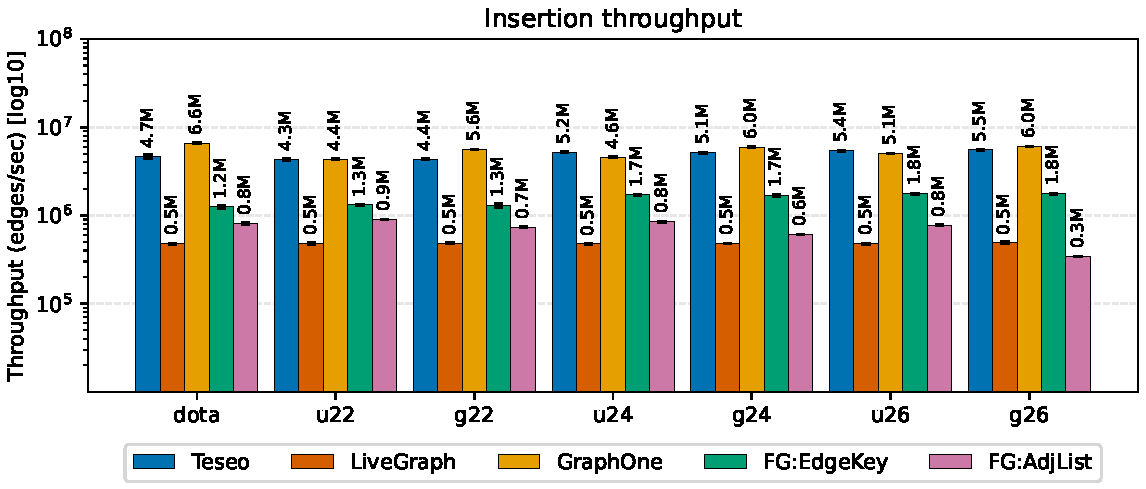
\includegraphics[width=\textwidth]{fig/dynamic/insertion_throughput_all.pdf}
  \caption{Dynamic graph operations:~peak insertion throughput across datasets when using optimal thread counts uncovered in \autoref{fig:dynamic-scaling}.}
  \label{fig:throughput-all}
\end{figure*}
%%%%%%%%%%%%%%%%%%%%%%%%%%%%%%%%%%%%%%%%%%%%%%%%%%%%%%%%%%%%%%%%%%%%%%%%%%%%%%%%

Under a sustained mixed workload (2.6\,B operations, ${\sim}$55\% insertions and ${\sim}$45\% deletions on graph500-24), the ranking changes (\autoref{fig:throughput-update}).
Teseo sustains 7.0\,M~ops/s, $\approx$30\% higher than its insertion-only rate.
Deletions create space for new insertions in an update-in-place structure such as the Teseo tree, so updates trigger fewer rebalances and leaf splits than a pure insertion stream does~\cite{teseo2021deLeo}.
\begin{figure*}[ht]
  \centering
  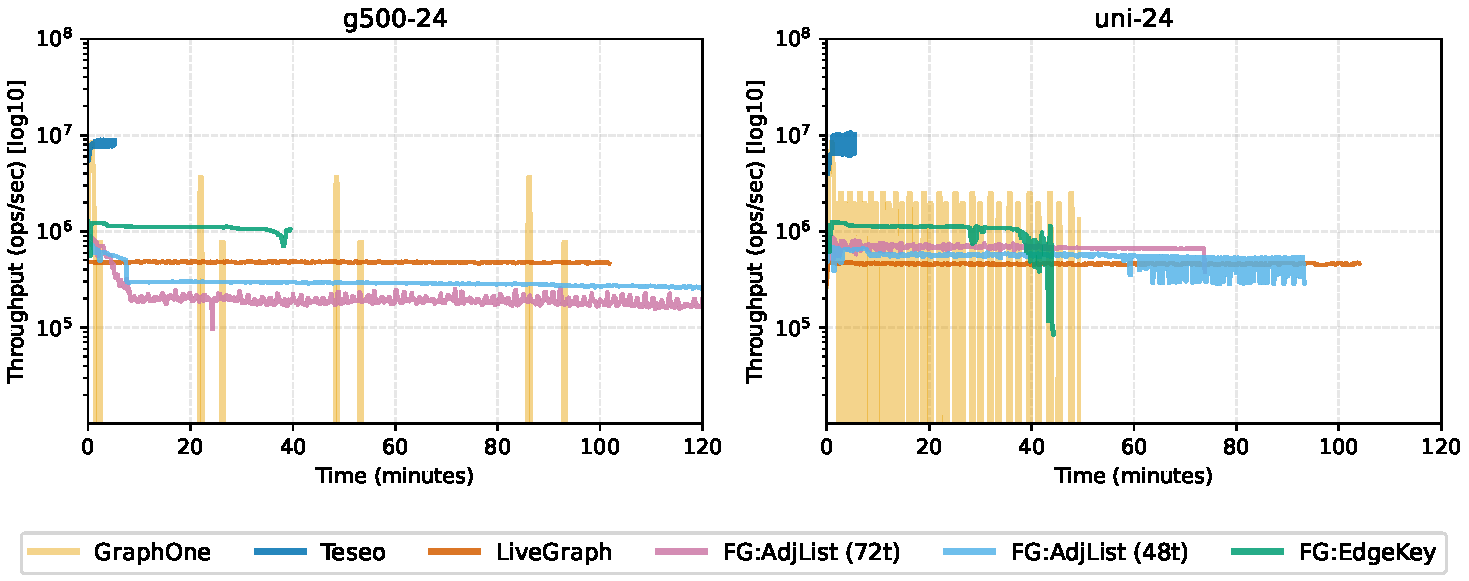
\includegraphics[width=\textwidth]{fig/dynamic/update_timeseries_combined.pdf}
  \caption{Update (insert/delete workload) throughput on graph500-24 and uniform-24. GraphOne throughput collapses for this workload. On uniform-24, \project{}'s AdjList at 72 threads outperforms its own 48-thread configuration because the uniform degree distribution reduces contention on individual adjacency records.}
  \label{fig:throughput-update}
\end{figure*}

GraphOne leads the insertion benchmark but collapses here to 0.05\,M~ops/s, a 114$\times$ drop.
The root cause is deletions: GraphOne's background archiver must locate the target edge to set a tombstone, and its append-only layout has no index for this lookup; on power-law graphs the resulting linear scan stalls the archiver and back-pressures writers.
\project{} EdgeKey sustains a modest 1.07\,M~ops/s, and LiveGraph sustains 0.42\,M~ops/s.
In LiveGraph, both edge additions and deletions are bottlenecked on finding the edge; the mutation itself is an append or a timestamp flip, respectively.
Vertex deletions simply tombstone the vertex block: incident edges are left in place and reclaimed by background compaction.
\project{}, by contrast, performs immediate cleanup: every incident edge is removed in a single transaction.
Under the Adjacency List layout, this requires rewriting each affected neighbor's packed list; under SplitEdgeKey, each edge is an independent B-tree row, so removal is a point delete.

The uniform-24 dataset, which lacks high-degree hub vertices, reveals how much degree skew drives update behavior.
GraphOne recovers to 0.87\,M~ops/s, only a 5.3$\times$ drop from its insertion rate, compared with the 114$\times$ collapse on graph500-24.
Without power-law hubs, the archiver's linear scan terminates quickly, so it no longer back-pressures writers.
Teseo sustains 6.0\,M~ops/s, roughly 14\% below its graph500-24 rate, likely because the more uniform key distribution triggers fewer in-place reuses of freed space.
LiveGraph is insensitive to degree distribution, sustaining 0.41\,M~ops/s (vs.\ 0.42 on graph500-24).
\project{} EdgeKey drops modestly to 0.95\,M~ops/s (from 1.07 on graph500-24), because each edge is an independent B-tree row, so degree skew has little effect on contention.
The largest shift is in Adjacency List: with 72 writer threads it reaches 0.58\,M~ops/s on uniform-24, outperforming its own 48-thread configuration (0.46\,M~ops/s) and reversing the thread-count ordering seen on graph500-24, where 48 threads (0.28\,M~ops/s) beat 72 (0.18\,M~ops/s).
Absent high-degree vertices, concurrent appends spread evenly across adjacency records instead of concentrating on a few hot lists, eliminating the contention that penalized the larger thread pool on the power-law graph.

\project{}'s two layouts present a clear tradeoff.
EdgeKey stores one B-tree row per edge; inserts are independent, carry no read-modify-write overhead, and incur almost no transaction aborts, scaling monotonically to 72~threads.
Adjacency List stores one record per vertex, so every edge insert appends to the source vertex's record.
Under power-law degree distributions, concurrent writers issue conflicting modifications to the records of high-degree vertices, producing a high rollback rate that limits peak throughput to ${\sim}$1.0\,M~edges/s at ${\sim}$48 threads, declining to ${\sim}$0.72\,M~edges/s at 72~threads.
On the other hand, Adjacency List performs better with 72 writer threads on the uniform-24 dataset because the absence of high-degree vertices reduces conflicts.

\section{Post-Ingestion Analytics}
\label{sec:eval:dynamic:analytics}
We next examine each system's analytics performance after ingest.
Once the insertion-only ingest of \autoref{sec:dynamic:ingest-update-tput} completes, we run BFS, PageRank~(PR), and weakly connected components~(WCC) in parallel across all physical cores on the resulting graph; no updates run during the analytics phase.
The results are in \autoref{tab:analytics-main}.

%%%%%%%%%%%%%%%%%%%%%%%%%%%%%%%%%%%%%%%%%%%%%%%%%%%%%%%%%%%%%%%%%%%%%%%%%%%%%%%%
\begin{table}[h!]
  \centering
  \begin{minipage}[t]{\columnwidth}
    \vspace{0pt}
    \centering
    % \footnotesize
    \setlength{\tabcolsep}{2pt}\renewcommand{\arraystretch}{1.0}
    \begin{tabular}{c l rrr | c l rrr}
    \toprule
    Graph & System & BFS & PR & WCC & Graph & System & BFS & PR & WCC \\
    \midrule
    \multirow{5}{*}{\rotatebox[origin=c]{90}{\small G500-22}} & FG AdjList & 0.16 & \textbf{0.18} & \textbf{0.20} & \multirow{5}{*}{\rotatebox[origin=c]{90}{\small Unif-22}} & FG AdjList & 0.14 & \textbf{0.17} & 0.11 \\
     & FG EdgeKey & 28.90 & 3.24 & 1.26 &  & FG EdgeKey & 23.20 & 3.19 & 0.71 \\
     & Teseo & \textbf{0.04} & 0.99 & 0.36 &  & Teseo & \textbf{0.07} & 1.44 & 0.50 \\
     & LiveGraph & 0.40 & 0.88 & 0.50 &  & LiveGraph & 0.14 & 0.68 & \textbf{0.06} \\
     & GraphOne & 3.82 & 4.47 & 13.20 &  & GraphOne & 3.84 & 4.60 & 16.00 \\
    \midrule
    \multirow{5}{*}{\rotatebox[origin=c]{90}{\small G500-24}} & FG AdjList & 0.37 & \textbf{0.81} & \textbf{0.48} & \multirow{5}{*}{\rotatebox[origin=c]{90}{\small Unif-24}} & FG AdjList & 0.35 & \textbf{0.93} & 0.62 \\
     & FG EdgeKey & 640.00 & 12.90 & 3.82 &  & FG EdgeKey & 547.00 & 12.70 & 3.75 \\
     & Teseo & \textbf{0.10} & 5.26 & 1.86 &  & Teseo & \textbf{0.16} & 8.60 & 2.76 \\
     & LiveGraph & 1.79 & 4.11 & 2.30 &  & LiveGraph & 0.57 & 5.89 & \textbf{0.25} \\
     & GraphOne & 4.10 & 7.37 & 67.80 &  & GraphOne & 4.04 & 9.97 & 95.80 \\
    \midrule
    \multirow{5}{*}{\rotatebox[origin=c]{90}{\small G500-26}} & FG AdjList & 1.29 & \textbf{5.52} & \textbf{3.70} & \multirow{5}{*}{\rotatebox[origin=c]{90}{\small Unif-26}} & FG AdjList & 1.05 & \textbf{9.91} & 4.24 \\
     & FG EdgeKey & t/o & 51.91 & 20.04 &  & FG EdgeKey & t/o & 51.43 & 14.36 \\
     & Teseo & \textbf{0.61} & 27.00 & 12.00 &  & Teseo & \textbf{0.55} & 50.20 & 15.60 \\
     & LiveGraph & 7.54 & 20.80 & 10.50 &  & LiveGraph & 2.08 & 32.80 & \textbf{0.95} \\
     & GraphOne & 4.86 & 19.90 & 346.00 &  & GraphOne & 5.99 & 40.20 & 401.00 \\
    \bottomrule
    \end{tabular}
    \vfill
    \caption{Cross-system Graphalytics kernel time (s), median over warm runs. The best time for each graph/algorithm appears in bold. FG = \project{}, PR = PageRank.}
    \label{tab:analytics-main}
  \end{minipage}
\end{table}
%%%%%%%%%%%%%%%%%%%%%%%%%%%%%%%%%%%%%%%%%%%%%%%%%%%%%%%%%%%%%%%%%%%%%%%%%%%%%%%%

Recall that, at this point, the in-memory baselines hold the graph only as a transient structure that will be lost if the system shuts down or crashes; there are neither redundant copies nor durable snapshots.

\newflag[new: cold-open cost]
\textbf{Cold-open cost.}
Unlike the purely in-memory baselines, \project{} stores the graph in \wt{}.
Immediately after ingestion, data resides as dirty pages in the buffer cache.
To ensure that Graphalytics kernels run on a stable, consistent, read-only view of the graph, \project{} forces a checkpoint and opens a set of per-thread read-only handles before the first kernel runs.
The checkpoint triggers \emph{reconciliation}, in which \wt{} walks every dirty page and reconciles its in-memory updates into the page images that constitute the queryable snapshot.
\autoref{tab:cold-open} reports the cost: reconciliation takes 59\,s on graph500-22 and grows to roughly 26\,min on the billion-edge graph500-26; opening the read-only handles adds at most 16\,s.
The competing systems incur no comparable cost, because they require no reconciliation step: LiveGraph's first runtime is nearly indistinguishable from its warm runtimes, and Teseo adds only a few seconds of cache warm-up.

%%%%%%%%%%%%%%%%%%%%%%%%%%%%%%%%%%%%%%%%%%%%%%%%%%%%%%%%%%%%%%%%%%%%%%%%%%%%%%%%
\begin{table}[t]
  \centering
  \setlength{\tabcolsep}{5pt}\renewcommand{\arraystretch}{1.05}
  \small
  \begin{tabular}{l rr rr}
  \toprule
   & \multicolumn{2}{c}{AdjList (s)} & \multicolumn{2}{c}{EdgeKey (s)} \\
  \cmidrule(lr){2-3}\cmidrule(lr){4-5}
  Graph & Reconcile & Open & Reconcile & Open \\
  \midrule
  G500-22 & 59 & 0.6 & 28 & 3.1 \\
  Unif-22 & 66 & 1.7 & 33 & 3.7 \\
  G500-24 & 298 & 2.1 & 219 & 11.9 \\
  Unif-24 & 284 & 5.8 & 234 & 14.3 \\
  G500-26 & 1{,}536 & 7.0 & --- & --- \\
  Unif-26 & 1{,}628 & 16.2 & --- & --- \\
  \bottomrule
  \end{tabular}
  \caption{Cold-open cost (seconds): forced checkpoint (reconciliation) and read-handle creation after ingestion, before the first analytics kernel runs.
  This is a one-time cost; subsequent kernels reuse the cached checkpoint.
  The EdgeKey rows at scale 26 are absent because we did not collect those runs.}
  \label{tab:cold-open}
\end{table}
%%%%%%%%%%%%%%%%%%%%%%%%%%%%%%%%%%%%%%%%%%%%%%%%%%%%%%%%%%%%%%%%%%%%%%%%%%%%%%%%

This cost is analogous to the preprocessing time we report for the out-of-core systems in \autoref{sec:eval:ooc}: in both cases a system must convert its ingested representation into one suitable for analytics before kernels can run.
The critical difference is what benefit this overhead brings.
The out-of-core systems build a single-purpose on-disk layout that is discarded after the benchmark; the in-memory baselines hold a transient structure that is lost on shutdown.
\project{}'s checkpoint produces a crash-recoverable snapshot: the graph is durable on disk and available for future queries without re-ingestion.
The cold open is therefore not overhead that vanishes with a better implementation, but the price \project{} pays \emph{once} to transition from a write-optimized buffer cache to a persistent, consistent read snapshot that subsequently serves analytics at in-memory speed.
Because subsequent kernels amortize it, \autoref{tab:analytics-main} reports steady-state time.

\project{} Adjacency List is the only system that delivers fast, stable performance across all three kernels and both graph families.
Teseo produces the best BFS runtime, 0.61\,s on graph500-26, but its PageRank and WCC degrade sharply at scale (27\,s and 12\,s respectively); on that same graph, \project{} Adjacency List runs PageRank in 5.5\,s, $4.9\times$ faster than Teseo, and WCC in 3.7\,s, $3.2\times$ faster.
LiveGraph is competitive on uniform WCC (0.95\,s) but scales poorly on power-law inputs.
GraphOne presents the starkest read-write contrast: it is the fastest inserter, yet its WCC collapses at graph500-26 to over $30\times$ slower than every other system, even though its BFS and PageRank remain comparable to LiveGraph and Teseo.
The ingest-optimized EdgeKey layout is orders of magnitude slower on analytics (640\,s for BFS on g500-24 versus 0.37\,s for AdjList), showing how much the choice of layout matters for analytics.

\textbf{Takeaway.}
Lacking a separate high-speed ingest path costs \project{} 3--5$\times$ on raw insertion relative to purpose-built in-memory systems, an expected and acceptable penalty.
This cost does not carry over to analytics, where \project{} Adjacency List matches or outperforms every baseline across all kernels and scales, while retaining the ability to persist and recover the graph, a feature that none of the in-memory systems provide.